
\subsection{ PaddleOCR }\

PaddleOCR is an open‑source, multi‑language OCR toolkit developed on the PaddlePaddle deep learning framework.

Here we use the PaddleOCR toolkit to perform image recognition on the LCD display of an intelligent electric meter. The model employed is a self‑trained model built upon the open‑source baseline. By annotating 1,000 photos of the LCD, we train with the PaddleOCR toolkit to generate our own model. Then, through calls to the OCR‑Server / OCR‑Client software, we enable automated testing of the intelligent electric meter’s LCD display.

\vspace{0.5cm}

\begin{lstlisting}
# create and use python virtual enviroment
conda activate paddleocr

# be sure  paddlepaddle-gpu is installed
python -m pip install paddlepaddle-gpu==3.0.0b1 -i https://pypi.tuna.tsinghua.edu.cn/simple

# modify the config file
cd /data/git/PaddleOCR/configs/rec
vi ppocr.yml

# copy trainning data to direcory train (1239 pics)
cp * /data/git/PaddleOCR/train_data/Lcd/train/

# copy testing data to directory test (131 pics)
cp * /data/git/PaddleOCR/train_data/Lcd/test/

# start training
python tools/train.py -c configs/rec/ppocr.yml

\end{lstlisting}

Some parameters from ppocr.yml : 

\begin{figure}[H]
    \begin{center}
        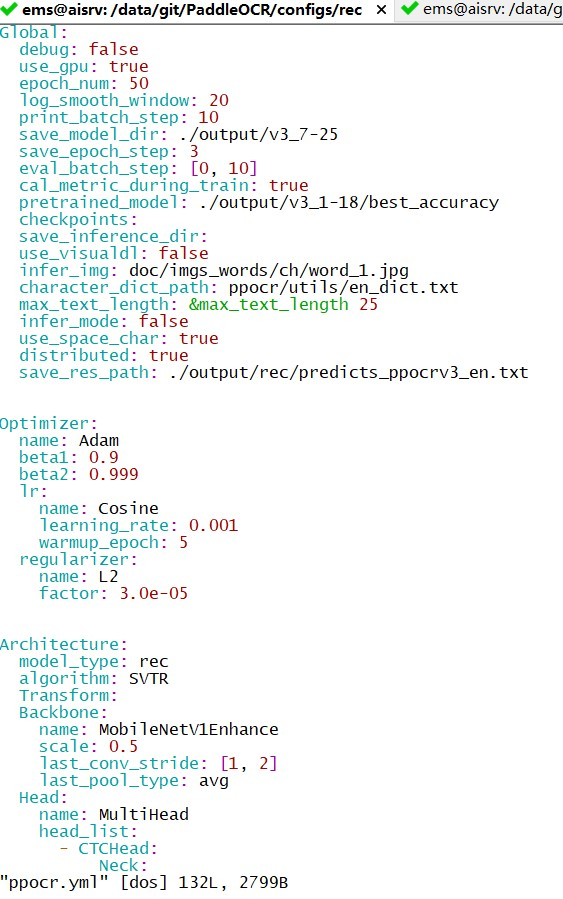
\includegraphics[width=.95\linewidth]{res/paddle-ocrconf.jpg}\\
        \caption{Part of ppocr.yml}\label{paddle-ocrconf}
    \end{center}
\end{figure}

Training process :

\begin{figure}[H]
    \begin{center}
        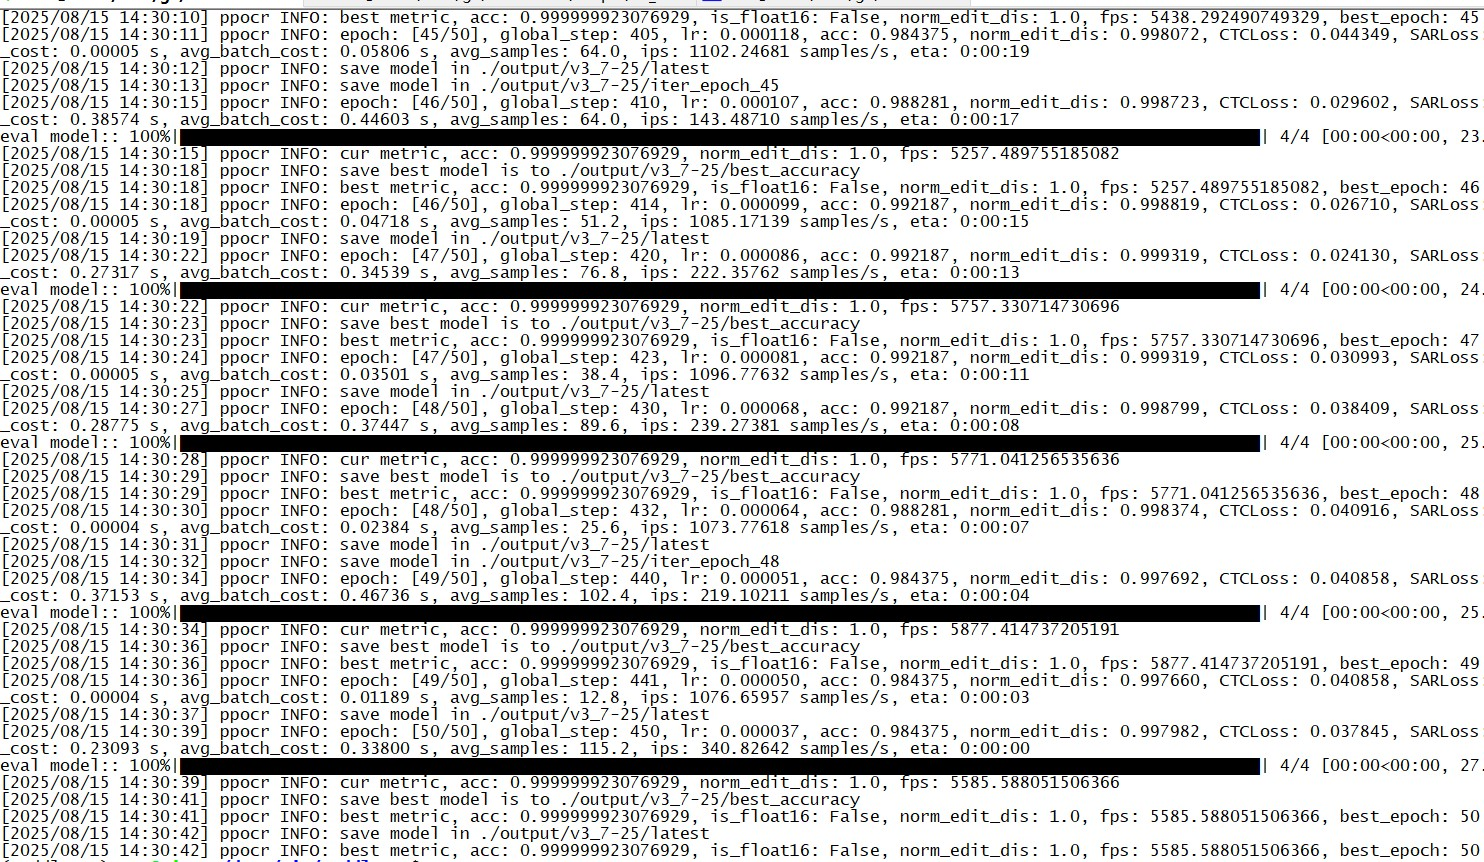
\includegraphics[width=.95\linewidth]{res/paddle-ocrtrain.jpg}\\
        \caption{50 epoch train process }\label{paddle-ocrtrain}
    \end{center}
\end{figure}